
\documentclass{article}
\usepackage{amsmath}
\usepackage{listings}
\usepackage{graphicx}
\usepackage[margin=1in]{geometry}
% \pagenumbering{gobble}
\usepackage{fancyhdr}
\setlength{\tabcolsep}{10pt}
\renewcommand{\arraystretch}{1.7}
 
\begin{document}

\pagestyle{fancy}
\fancyhf{}
\renewcommand{\headrulewidth}{0pt}
\fancyfoot[CE,CO]{F - \thepage}

\section*{\hfil F. \textit{Jomblo} dan \textit{Taken}\hfil}

% \begin{center}
% \begin{tabular}{ |cc| } 
%  \hline
%  Time Limit & 2 detik \\
%  \hline 
%  Memory Limit & 256 MB \\
%  \hline
% \end{tabular}
% \end{center}

\subsection*{Deskripsi}

\par\noindent Ada dua tipe orang di dunia ini, yang \textit{taken} dan yang \textit{jomblo}. Bocan yang \textit{jomblo} sangat kesal jika melihat orang yang \textit{taken}. Karena tidak mau Bocan sedih, Turpa ingin membunuh semua orang \textit{taken} dengan bom. Namun, Turpa hanya mempunyai satu bom.
\newline
\par\noindent Di ITB, ada $N$ orang \textit{taken} dan M orang \textit{jomblo}. Mereka semua berada di kampus ITB yang dipetakan ke titik koordinat kartesian. Meskipun semua orang \textit{taken} harus musnah, Turpa tidak mau menumpahkan darah orang \textit{jomblo}. Untuk itu, ia dapat memaksa beberapa orang pindah ke koordinat lain. Namun agar tidak dicurigai, ia ingin memindahkan orang sesedikit mungkin.
\newline
\par\noindent Turpa ingin tahu berapa jumlah orang minimum yang perlu dipindahkan supaya terdapat lokasi bom dan semua orang \textit{taken} tidak berada di luar radius bom, serta semua orang \textit{jomblo} tidak berada di dalam radius bom. Orang yang ada tepat di radius bom hanya akan terbunuh bila ia \textit{taken}. Ingat jika radius bom Turpa sangat fleksibel dan dapat ia ubah sesuka hati. Sebelum Turpa melakukan pemindahan, tidak ada dua orang yang berada pada posisi yang
sama. Setiap orang dapat dipindahkan ke posisi manapun, posisi pemindahan tidak harus bilangan bulat dan setelah pemindahan bisa saja terdapat dua orang dengan posisi yang sama.

\subsection*{Format Masukan}

\par\noindent Baris pertama berisi dua buah bilangan bulat $N$ dan $M$.
\par\noindent $N$ baris selanjutnya berisi 2 bilangan bulat $x$ dan $y$, yang menyatakan koordinat orang \textit{taken}.
\par\noindent $M$ baris selanjutnya berisi 2 bilangan bulat $x$ dan $y$, yang menyatakan koordinat orang \textit{jomblo}.

\subsection*{Format Keluaran}

\par\noindent Sebuah baris berisi bilangan, jumlah orang minimum yang dipindahkan supaya memenuhi kriteria Turpa.

\subsection*{Contoh Masukan 1}

\begin{lstlisting}
3 1
0 0
10 0
5 10
5 5
\end{lstlisting}

\subsection*{Contoh Keluaran 1}

\begin{lstlisting}
1
\end{lstlisting}

\subsection*{Contoh Masukan 2}

\begin{lstlisting}
2 2
0 1
0 -1
1 0
-1 0
\end{lstlisting}

\subsection*{Contoh Keluaran 2}

\begin{lstlisting}
0
\end{lstlisting}

\subsection*{Batasan}

\begin{itemize}
  \item $0 \leq N,M \leq 200$
  \item $-10^3 \leq x, y \leq 10^3$
  \item Pada awalnya tidak ada dua orang yang berada pada posisi yang sama.
\end{itemize}

\subsection*{Penjelasan}

\par\noindent Contoh letak bom untuk contoh masukan 1:

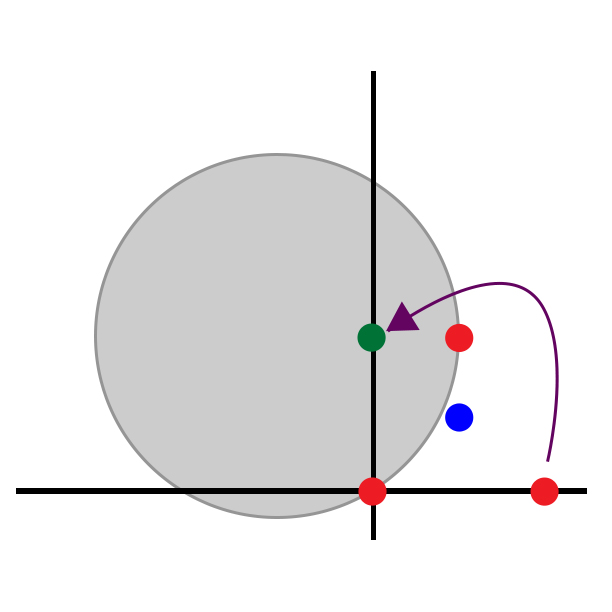
\includegraphics[width=5cm]{sample-1}

\par\noindent Kita dapat menaruh bom supaya memiliki ledakan seperti gambar (lingkaran abu-abu) dan memindahkan titik di $(10,0)$ ke titik berwarna hijau.

\par\noindent Ada beberapa cara lain, namun semuanya butuh memindahkan tidak kurang dari $1$ titik.

\par\noindent Contoh letak bom untuk contoh masukan 2:

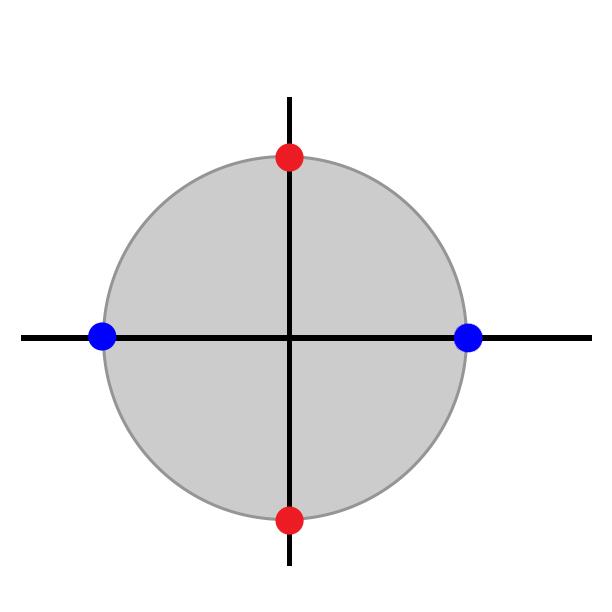
\includegraphics[width=5cm]{sample-2}

\par\noindent Kita hanya dapat menaruh bom di $(0,0)$ dengan radius $1$ satuan. Perhatikan bahwa orang yang ada di garis radius boleh \textit{jomblo} dan boleh \textit{taken}.

\end{document}
